\subsection{The Sine Rule}
\begin{theorybox}{Notes}

The vertices (corners) of any figure are labelled using capital letters. In a triangle, the sides are labelled using the lower case letter of the opposing vertex.

\begin{center}
    \begin{tikzpicture}[scale=0.65]
        \draw (0,0) node[below left]{$A$} -- node[below right]{$c$}(6,2)node[right]{$B$} -- node[above right]{$a$} (2,5) node[above]{$C$} -- node[left]{$b$}cycle;
    \end{tikzpicture}
\end{center}

The sine rule states that $\dfrac{a}{\sin A}=\dfrac{b}{\sin B}=\dfrac{a}{\sin C}$.
\vskip5mm
When finding an unknown angle, we can use the form $\dfrac{\sin A}{a}=\dfrac{\sin B}{b}=\dfrac{\sin C}{c}$.

\end{theorybox}

\begin{pfbox}{Proof}

The diagram below shows triangle $ABC$ where $AC=b$, $BC=a$ and point $M$ lies on $AB$ such that $AB \perp CM$.
\begin{center}
    \begin{tikzpicture}
        \draw (0,0) node[below left]{$A$} -- (7,0)node[right]{$B$} -- node[above right]{$a$} (4,3) node[above]{$C$} -- node[above left]{$b$}cycle;
        \draw[dashed] (4,3) -- (4,0) node[below]{$M$};
        \draw (3.75,0) -- (3.75,0.25) -- (4,0.25);
    \end{tikzpicture}
\end{center}

From $\triangle ACM$, $\sin A = \dfrac{CM}{b} \Rightarrow CM = b \sin A$.
\vskip5mm
Similarly in $\triangle BCM$, $\sin B = \dfrac{CM}{a} \Rightarrow CM = a \sin B$.
\vskip5mm
Equating these expressions for $CM$ gives:
\begin{align*}
    b \sin A &= a \sin B \\
    \therefore \dfrac{a}{\sin A}&=\dfrac{b}{\sin B}
\end{align*}
This process can be repeated involving vertex $C$ and its opposing side to give the sine rule as it is conventionally stated.
\end{pfbox}


%% Worked Examples

\begin{examplecz}{Finding an unknown side}

In $\triangle ABC$, $AC=21$\,cm, $BC=x$\,cm, $\angle CAB=38^{\circ}$ and $\angle CBA=43$ as shown.
\begin{center}
    \begin{tikzpicture}
        \coordinate[label=left: $A$] (A) at (0,0);
        \coordinate[label=right: $B$] (B) at (6.5,-1);
        \coordinate[label=above: $C$] (C) at (4,2);
        \draw (A) -- (B) -- node[above right]{$x$\,cm} (C) -- node[above left]{$21$\,cm}cycle;
        \tkzLabelAngle[pos=1.2](C,B,A){$43^{\circ}$};
        \tkzLabelAngle[pos=1.2](B,A,C){$38^{\circ}$};        
    \end{tikzpicture}
\end{center}
Find the value of $x$, correct to two decimal places.
\tcblower
\textbf{Solution:}
\vspace*{40mm}
\begin{comment}
\begin{align*}
    \dfrac{x}{\sin 38^{\circ}} &= \dfrac{21}{\sin 43^{\circ}} \\
    x &= \dfrac{21\times \sin 38^{\circ}}{\sin 43^{\circ}} \\
    \therefore x &= 18.96\,\text{cm}
\end{align*}
\end{comment}

\end{examplecz}

\vspace*{5mm}


\begin{examplecz}{Finding an unknown angle}

In $\triangle ABC$ shown, $AB=10\,\text{cm}$, $BC=7\,\text{cm}$ and $\angle ACB=110^{\circ}$ and $\angle BAC=\theta$.
\begin{center}
    \begin{tikzpicture}
        \coordinate[label=below left: $A$] (A) at (0,0);
        \coordinate[label=right: $B$] (B) at (6.5,1.5);
        \coordinate[label=above: $C$] (C) at (2,3);
        \draw (A) -- node[below]{$10$\,cm}(B) -- node[above right]{$7$\,cm} (C) -- cycle;
        \tkzLabelAngle[pos=0.7](A,C,B){$110^{\circ}$};
        \tkzLabelAngle[pos=1](B,A,C){$\theta$};        
    \end{tikzpicture}
\end{center}
Find the value of $\theta$, correct to two decimal places.
\tcblower
\textbf{Solution:}
\vspace*{40mm}
\begin{comment}
\begin{align*}
    \dfrac{\sin \theta}{7} &= \dfrac{\sin 110 ^{\circ}}{10} \\
    \sin \theta &= \dfrac{7 \sin 110^{\circ}}{10} \\
    \therefore \theta &= \sin ^{-1} \left(\dfrac{7 \sin 110^{\circ}}{10}  \right) \\
    &= 41.13^{\circ}
\end{align*}
\end{comment}

\end{examplecz}

%% Self-paced Questions 

\begin{examplecz}{}

Triangle $HIJ$ has sides $IJ=14$\,cm and $HJ=x$\,cm. $\angle JHI=37^{\circ}$ and $\angle HIJ=52^{\circ}$ as shown. 
\begin{center}
    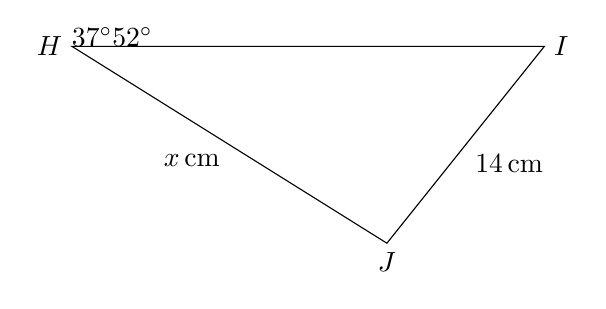
\begin{tikzpicture}
        \coordinate[label=left: $H$] (H) at (0,0);
        \coordinate[label=right: $I$] (I) at (6,0);
        \coordinate[label=below: $J$] (J) at (4,-2.5);
        \draw (H) -- (I) -- node[below right]{$14$\,cm} (J) -- node[below left]{$x$\,cm} cycle;
        \tkzLabelAngle[pos=1.4](J,H,I){$37^{\circ}$};
        \tkzLabelAngle[pos=1.1](H,I,J){$52^{\circ}$};        
    \end{tikzpicture}
\end{center}
Find the value of $x$, correct to one decimal place.
\tcblower
\textbf{Solution:}
\vspace*{4.5cm}
%\begin{align*}
%    \dfrac{\sin \theta}{13} &= \dfrac{\sin 89 ^{\circ}}{25} \\
%    \sin \theta &= \dfrac{13 \sin 89^{\circ}}{25} \\
%    \therefore \theta &= \sin ^{-1} \left(\dfrac{13 \sin 89^{\circ}}{25}  \right) \\
%    &= 31^{\circ}
%\end{align*}
\end{examplecz}

\vspace{5mm}

\begin{examplecz}{}
In $\triangle PQR$ shown, $PQ=25$\,cm, $PR=13$\,cm, $\angle PRQ=89^{\circ}$ and $\angle PQR=\theta$.
\begin{center}
    \begin{tikzpicture}
        \coordinate[label=left: $P$] (P) at (0,0);
        \coordinate[label=right: $Q$] (Q) at (6,0);
        \coordinate[label=above: $R$] (R) at (2,3);
        \draw (P) -- node[below]{$25$\,cm}(Q) -- (R) -- node[above left]{$13$\,cm} cycle;
        \tkzLabelAngle[pos=0.7](P,R,Q){$89^{\circ}$};
        \tkzLabelAngle[pos=1](R,Q,P){$\theta$};        
    \end{tikzpicture}
\end{center}
Find the value of $\theta$, correct to the nearest degree.
\tcblower
\textbf{Solution:}
\vspace*{4.5cm}
%\begin{align*}
%    \dfrac{\sin \theta}{13} &= \dfrac{\sin 89 ^{\circ}}{25} \\
%    \sin \theta &= \dfrac{13 \sin 89^{\circ}}{25} \\
%    \therefore \theta &= \sin ^{-1} \left(\dfrac{13 \sin 89^{\circ}}{25}  \right) \\
%    &= 31^{\circ}
%\end{align*}
\end{examplecz}

\begin{examplecz}{}
In $\triangle XYZ$, $XY=20.8$\,cm, $YZ=17.6$\,cm, $\angle XZY=26^{\circ}$ and $\angle XYZ=\theta$ as shown.
\begin{center}
    \begin{tikzpicture}
        \coordinate[label=left: $X$] (X) at (0,0);
        \coordinate[label=right: $Y$] (Y) at (5,0);
        \coordinate[label=above: $Z$] (Z) at (7,3);
        \draw (X) -- node[below]{$20.8$\,cm}(Y) -- node[below right]{$17.6$\,cm} (Z) -- cycle;
        \tkzLabelAngle[pos=1.3](X,Z,Y){$26^{\circ}$};
        \tkzLabelAngle[pos=0.5](Z,Y,X){$\theta$};        
    \end{tikzpicture}
\end{center}
Find the value of $\theta$, correct to the nearest minute.
\tcblower
\textbf{Solution:}
\vspace*{5cm}
%\begin{align*}
%    \dfrac{\sin \theta}{13} &= \dfrac{\sin 89 ^{\circ}}{25} \\
%    \sin \theta &= \dfrac{13 \sin 89^{\circ}}{25} \\
%    \therefore \theta &= \sin ^{-1} \left(\dfrac{13 \sin 89^{\circ}}{25}  \right) \\
%    &= 31^{\circ}
%\end{align*}
\end{examplecz}




\vfill
\begin{Qbox}{}
    From \textit{CambridgeMaths Year 11 Mathematics Extension 1}:
    \begin{itemize}
        \item Exercise 6I: 1, 2, 3, 5 and 12
    \end{itemize}
\end{Qbox}